\documentclass[UTF8, a4paper, 12pt]{ctexart}

\usepackage{graphicx}
\usepackage{booktabs}
\usepackage{geometry}
\usepackage{amsmath}
\usepackage{hyperref}
\usepackage{array}
\usepackage{float}

\geometry{left=2.5cm,right=2.5cm,top=2.2cm,bottom=2.3cm}

\linespread{1.5}

\title{Python 强化学习迷宫程序设计（第三次作业）}
\author{通信2301 毛锦翔}
\date{}

\pagestyle{plain}
\begin{document}
\maketitle

\section*{摘要}

本实验围绕离散迷宫环境中的强化学习寻路任务展开，目标是在设计的 5x5 网格迷宫中，使用 Q-Learning 训练智能体从固定起点到达终点。系统包含环境建模、奖励机制设计、Q-table 学习与 Tkinter 可视化演示等模块。算法采用 epsilon-greedy 策略进行探索与利用，结合学习率、折扣因子与探索衰减策略实现稳定收敛。实验过程中可实时观察智能体从随机探索逐步收敛到稳定路径的过程，并支持演示当前最优策略路径。结果表明，所实现的 Q-Learning 能在该迷宫任务上形成可行的最优或近似最优路径，验证了算法在离散状态空间中的有效性。

\textbf{关键词：}强化学习；Q-Learning；迷宫寻路；Q-table；可视化

\section{任务背景与目标}

迷宫寻路是强化学习的经典入门任务，能够清晰体现状态、动作、奖励与策略之间的关系。通过该实验可以掌握 Q-Learning 的更新逻辑和 epsilon-greedy 策略的作用，并理解探索与利用的平衡机制。

本次作业目标包括：
\begin{itemize}
  \item 设计离散迷宫环境与奖励机制，定义状态与动作空间。
  \item 实现 Q-Learning 智能体与 Q-table 更新。
  \item 构建训练主循环，实现回合控制与探索率衰减。
  \item 通过 Tkinter 可视化训练过程并演示最优路径。
\end{itemize}

\section{系统设计与方法}

\subsection{迷宫环境建模}

迷宫采用 5x5 网格，坐标按课程示意图使用 1-based 说明，程序内部使用 0-based 坐标。
\begin{itemize}
  \item 起点：$[2,1]$(内部坐标 $(1,0)$)
  \item 终点：$[5,5]$(内部坐标 $(4,4)$)
  \item 障碍：$[3,3]$、$[3,4]$、$[3,5]$、$[4,3]$
  \item 特殊跃迁：从 $[2,4]$ 进入后跳到 $[4,4]$，奖励 $+5$
  \item 动作空间：上、下、左、右($0,1,2,3$)
\end{itemize}

\begin{figure}[H]
  \centering
  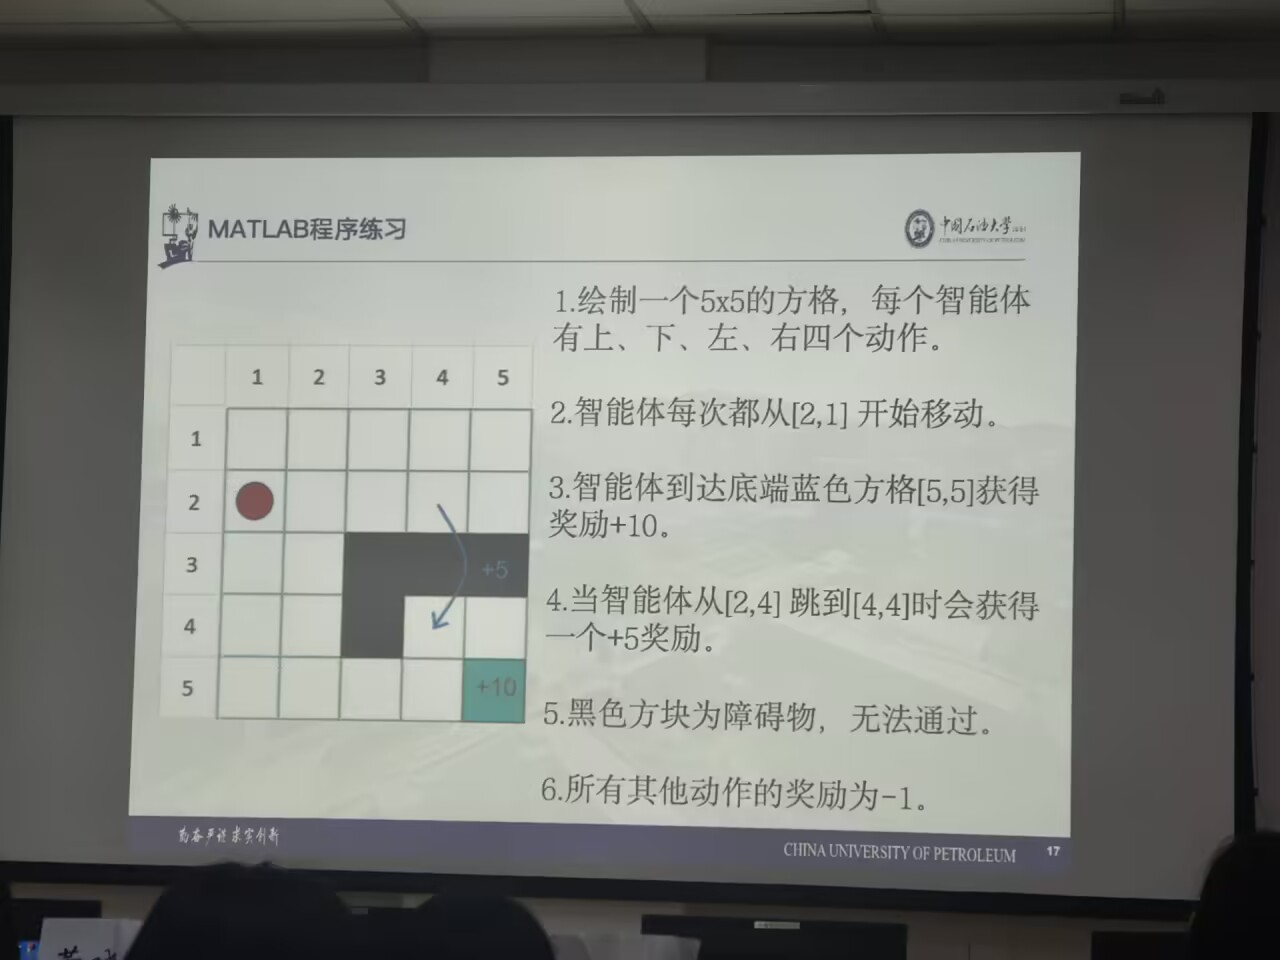
\includegraphics[width=0.9\linewidth]{具体要求.jpg}
  \caption{迷宫设置与奖励规则（课程要求截图）}
\end{figure}

状态采用二维坐标 $(r,c)$ 表示智能体在网格中的位置，属于有限离散状态空间。环境在每一步根据动作执行状态转移，并输出下一状态、即时奖励以及是否结束回合（到达终点）。这样将迷宫问题标准化为“离散状态-离散动作”的 MDP，方便直接应用表格型 Q-Learning。

\subsection{奖励设计}

奖励规则如下：
\begin{itemize}
  \item 到达终点：$+10$，回合结束
  \item 触发特殊跃迁：$+5$，继续回合
  \item 撞墙/越界/障碍阻挡：$-1$，位置不变
  \item 其余动作：$-1$
\end{itemize}

为便于实现与分析，将奖励函数写成分段形式。设当前状态为 $s$，动作 $a$ 执行后得到下一状态 $s'$，即时奖励 $r(s,a,s')$ 定义为：
\begin{equation}
r(s,a,s')=
\begin{cases}
10, & s' = \text{goal} \\
5, & s' = \text{jump\_to} \\
-1, & s' = s \ \text{且动作为越界/障碍} \\
-1, & \text{其他可达状态}
\end{cases}
\end{equation}

其中 \text{goal} 对应终点 $[5,5]$，\text{jump\_to} 对应特殊跃迁落点 $[4,4]$。该设计体现了以下考虑：
\begin{itemize}
  \item 终点奖励设置为 $+10$，显著高于一步代价，保证到达终点是主要优化目标。
  \item 特殊跃迁奖励 $+5$ 作为“局部吸引”，引导智能体在可行路径中优先触发跳跃，以减少总步数并提升回报。
  \item 统一步进代价 $-1$（包含无效动作与普通移动）抑制无目的探索，鼓励更短路径。
  \item 对撞墙/越界/障碍同样给出 $-1$，使无效动作在价值上显式劣化，有助于 Q-table 更快区分可行动作与不可行动作。
\end{itemize}

该奖励函数属于“稀疏目标奖励 + 密集步进惩罚”的组合形式，在小型离散迷宫中能够稳定推动策略收敛，同时使最优路径与最大奖励方向保持一致。

\subsection{Q-Learning 更新公式}

Q-Learning 的核心更新公式为：
\begin{equation}
Q(s,a) \leftarrow Q(s,a) + \alpha \left[r + \gamma \max_{a'} Q(s',a') - Q(s,a)\right]
\end{equation}

其中 $\alpha$ 为学习率，$\gamma$ 为折扣因子。策略采用 epsilon-greedy：以概率 $\epsilon$ 随机探索，以 $1-\epsilon$ 选择当前最优动作，并在回合结束后进行探索率衰减。

\subsection{训练流程与回合控制}

训练过程以回合为单位进行。在每个回合中，智能体从固定起点开始，不断执行动作并更新 Q-table，直到到达终点或达到最大步数。回合结束后，对探索率进行衰减并重置环境。训练流程要点如下：
\begin{itemize}
  \item 读取当前状态 $s$，按 epsilon-greedy 选择动作 $a$。
  \item 环境执行 $a$，得到 $s'$、$r$ 与终止标志 $done$。
  \item 按 Q-Learning 公式更新 $Q(s,a)$。
  \item 若 $done$ 或步数超限，则结束回合并进行探索率衰减。
\end{itemize}

\subsection{可视化与交互}

系统使用 Tkinter 提供图形界面，实现训练过程的实时展示与交互控制：
\begin{itemize}
  \item 开始/暂停/重置训练
  \item 调节训练速度（延迟时间）
  \item 演示当前 Q-table 下的最优路径
\end{itemize}

图例中使用颜色区分智能体、障碍、终点与特殊跃迁位置，便于观察策略演化。

\section{实验设置}

\subsection{实现环境}

系统基于 Python 编写，采用 Tkinter 作为可视化框架，模块划分清晰：
\begin{itemize}
  \item \texttt{maze\_env.py}：迷宫环境与奖励规则
  \item \texttt{rl\_brain.py}：Q-Learning 智能体与 Q-table
  \item \texttt{main.py}：GUI 与训练主循环
\end{itemize}

\subsection{核心参数}

默认配置如下（可在源码中调整）：
\renewcommand{\arraystretch}{1.3}
\begin{table}[H]
\centering
\begin{tabular}{>{\centering\arraybackslash}p{4cm} >{\centering\arraybackslash}p{6cm}}
\multicolumn{1}{c}{\textbf{配置项}} & \multicolumn{1}{c}{\textbf{参数值}} \\
\midrule
学习率 $\alpha$ & 0.1 \\
折扣因子 $\gamma$ & 0.9 \\
初始探索率 $\epsilon$ & 1.0 \\
最小探索率 & 0.05 \\
探索衰减系数 & 0.995 \\
每回合最大步数 & 200 \\
\bottomrule
\end{tabular}
\caption{Q-Learning 核心参数}
\end{table}
\renewcommand{\arraystretch}{1}

\section{实验结果与分析}


训练初期，Q-table 近似为零，智能体以随机探索为主，表现为路径长度较长、回报波动大，且经常出现撞墙或无效动作。随着回合推进，Q 值开始区分可行动作与不可行动作，探索率逐步衰减，策略逐渐从“广泛探索”转向“稳定利用”。

在最初的训练阶段，由于 Q-table 尚未积累有效经验，智能体对每个状态下的动作价值估计几乎一致，导致动作选择高度随机。这一时期，智能体常常在迷宫中反复尝试各种路径，甚至多次进入死胡同或在障碍物附近徘徊，整体表现为到达终点的步数较多、回合奖励波动较大。此时，Q-table 的更新主要依赖于环境反馈的即时奖励，尤其是撞墙、越界等无效动作的负奖励，有助于智能体逐步识别并规避这些低价值行为。

随着训练回合的增加，Q-table 中各状态-动作对的价值逐步拉开差距。智能体在经历多次失败和尝试后，能够通过 Q 值的累积效应，逐步学会避开障碍和无效区域，优先选择那些历史上带来较高回报的动作。探索率 epsilon 也在每回合后按设定衰减，进一步推动策略从“广泛探索”向“稳定利用”转变。此时，智能体到达终点的平均步数明显减少，回合奖励趋于稳定。

从可视化过程可观察到两个阶段性特征：第一阶段智能体尝试多条路线并频繁回退；第二阶段在高价值状态附近形成稳定动作偏好，路径趋于固定。特殊跃迁位置的 $+5$ 奖励提供了明确的局部吸引，促使智能体在可行路径中优先走向该位置，从而降低总步数并提高回报。

具体来看，训练过程可分为两个明显阶段：
\begin{itemize}
  \item \textbf{探索主导阶段}：智能体尝试多条不同路线，频繁回退或在障碍附近徘徊，Q-table 变化剧烈，策略尚未收敛。
  \item \textbf{利用主导阶段}：随着 Q-table 收敛，智能体在高价值状态附近形成稳定动作偏好，路径趋于固定，能够高效到达终点。
\end{itemize}

值得注意的是，特殊跃迁位置的 $+5$ 奖励在策略形成过程中起到了“局部吸引”的作用。智能体在多次尝试后，逐渐学会优先走向该位置，利用跃迁获得更高回报。这不仅缩短了到达终点的步数，也提升了整体策略的回报率，体现了奖励设计对学习效果的直接影响。



总体上，Q-Learning 在该离散迷宫任务中能够稳定收敛，训练过程可视化清晰展示了从探索到利用的策略演化过程，且“最优路径演示”功能可稳定输出到达终点的路径，说明策略已基本学成。

\section{系统展示与功能}

系统提供如下功能：
\begin{itemize}
  \item 训练过程实时可视化
  \item 训练速度可调
  \item 一键演示当前最优策略路径
  \item 支持重置训练与 Q-table
\end{itemize}

界面上方提供控制区与状态信息区，能够显示当前回合、步数、累计回报与探索率，便于观察学习进度。画布区域实时绘制迷宫、障碍、起点终点与智能体位置，并对特殊跃迁进行箭头标注，使关键奖励机制直观可见。

\subsection{GUI界面说明与最优路径演示}
\begin{figure}[H]
  \centering
  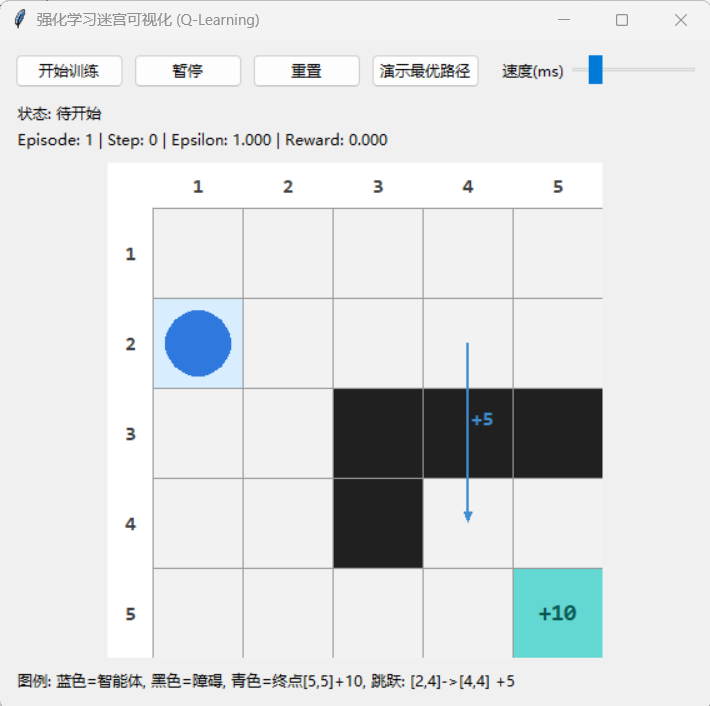
\includegraphics[width=0.95\linewidth]{GUI界面.png}
  \caption{迷宫强化学习系统的GUI界面截图}
\end{figure}

如上图所示，系统采用基于Tkinter的图形用户界面，整体布局简洁直观，主要分为以下几个区域：
\begin{itemize}
  \item \textbf{控制区}：位于界面上方，包含“开始训练”“暂停”“重置”“演示最优路径”等按钮，便于用户灵活控制训练流程。
  \item \textbf{参数与状态显示区}：实时显示当前回合数、步数、累计奖励、探索率等关键信息，帮助用户跟踪训练进度和策略收敛情况。
  \item \textbf{迷宫可视化区}：中央画布动态绘制迷宫网格、障碍、起点、终点、特殊跃迁（带箭头和奖励标注）以及智能体当前位置。训练过程中，智能体的移动和策略演化会实时反映在该区域。
  \item \textbf{图例与说明区}：界面底部提供颜色图例和特殊规则说明，帮助理解不同元素的含义。
\end{itemize}


用户可通过调整训练速度滑块，观察不同速度下智能体的学习过程。训练过程中，界面会自动刷新状态和迷宫布局，便于直观感受 Q-Learning 策略从探索到收敛的全过程。

\begin{figure}[H]
  \centering
  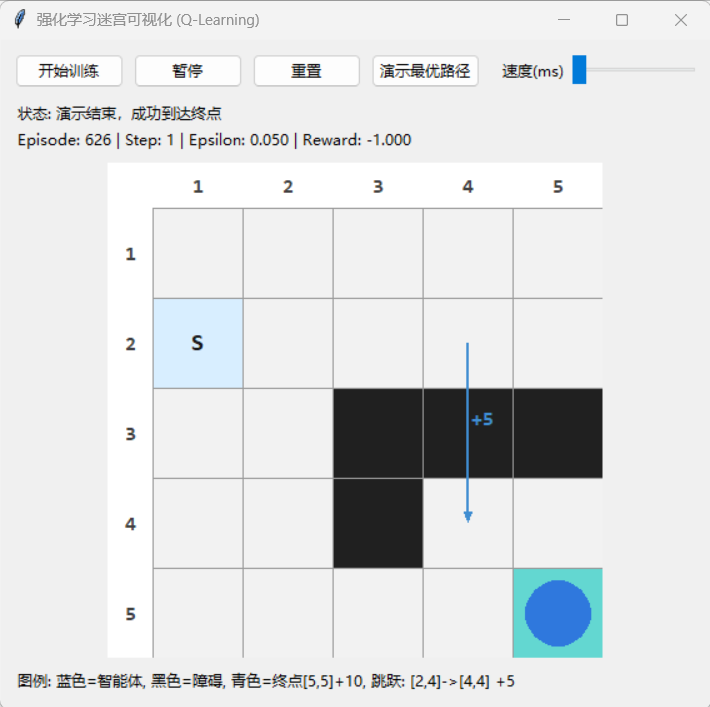
\includegraphics[width=0.8\linewidth]{最优路径.png}
  \caption{演示当前 Q-table 下智能体走最优路径的界面截图}
\end{figure}

如上图所示，系统支持一键演示当前 Q-table 下的最优路径。训练收敛后，智能体能够稳定地从起点出发，沿最优或近似最优路径到达终点，并在可行情况下优先触发特殊跃迁获得更高回报。该功能直观展示了 Q-Learning 策略的学习效果和最终表现。

运行方式：在目录下执行
\texttt{python main.py}

\section{局限与改进方向}
\begin{itemize}
  \item 迷宫规模较小，状态空间有限，难以体现更复杂策略。
  \item 使用表格型 Q-Learning，难以扩展到连续或大规模状态空间。
  \item 可尝试引入 SARSA 或 DQN 以进行算法对比。
  \item 可增加奖励设计与障碍布局的多样性，提升任务难度与泛化性。
\end{itemize}

\section{结论}

本实验以 Q-Learning 算法为核心，系统性地实现了一个可视化的迷宫强化学习平台。通过对 5x5 网格迷宫环境的建模、奖励函数的精心设计、Q-table 的动态更新与策略收敛过程的可视化展示，全面验证了 Q-Learning 在离散状态空间下的有效性和实用性。

实验结果表明，合理的奖励机制（如终点高奖励、特殊跃迁奖励、统一步进惩罚）能够显著加速策略收敛，引导智能体形成高效路径。训练过程中，智能体从完全随机探索逐步过渡到稳定利用，最终能够多次稳定到达终点并优先选择最优路线，充分体现了强化学习“试错—积累—优化”的本质。

本项目还通过 Tkinter 图形界面实现了训练过程的实时可视化和交互操作，极大提升了实验的直观性和可操作性。用户可灵活调整参数、观察策略演化、演示最优路径，为理解 Q-Learning 算法提供了良好的实验平台。

展望未来，迷宫强化学习系统可在以下方向进一步拓展和优化：
\begin{itemize}
  \item \textbf{算法层面}：引入 SARSA、DQN 等其他强化学习算法，比较不同方法在复杂环境下的表现。
  \item \textbf{环境扩展}：增加迷宫规模、障碍类型或动态环境，考察算法的泛化能力和鲁棒性。
  \item \textbf{奖励机制优化}：尝试稀疏奖励、分层奖励等设计，分析奖励结构对学习效率和策略质量的影响。
  \item \textbf{可视化与交互}：丰富界面功能，如路径回放、Q-table 热力图展示、训练日志导出等，提升用户体验。
  \item \textbf{实际应用}：将强化学习方法迁移到更具挑战性的实际问题，如机器人路径规划、自动驾驶等。
\end{itemize}

综上，本实验不仅加深了对 Q-Learning 强化学习原理与实现细节的理解，也为后续深入研究和应用更复杂强化学习算法打下了坚实基础。

\section{主要代码说明}

\subsection{maze\_env.py}
实现迷宫环境状态转移与奖励规则，包含边界检测、障碍判断、终点判定与特殊跃迁逻辑。

\subsection{rl\_brain.py}
实现 Q-Learning 智能体，维护 Q-table，并提供 epsilon-greedy 动作选择、更新与探索率衰减。

\subsection{main.py}
负责 GUI 构建与训练主循环控制，完成可视化绘制、训练步骤推进、回合切换与路径演示。

\subsection{run.py}
作为入口脚本，调用 \texttt{main.py} 中的启动函数。

\end{document}
